\documentclass[a4paper,12pt]{article} % Тип документа



\usepackage{graphicx}
\graphicspath{{pictures/}}
\DeclareGraphicsExtensions{.pdf,.png,.jpg}
\usepackage{multirow}

% Русский язык
\usepackage[T2A]{fontenc}
\usepackage[utf8]{inputenc}
\usepackage[english,russian]{babel}

% Математика
\usepackage{amsmath,amsfonts,amssymb,amsthm,mathtools} 


\usepackage{wasysym}

%Заговолок
\author{Маллаев Руслан}
\title{Лабораторная работа №1.4.5}
\date{11 октября 2020 г.}

\begin{document} % Начало документа

\maketitle
\newpage
 
 \textbf{Цель работы:} исследование зависимости частоты колебаний струны 
 
 от величины натяжения, нахождение гармоник и собственных частот колебания струны, а также условий установления стоячей вол-
 
 ны, получающейся в результате сложения волн, идущих в противопо-
 
 ложных направлениях.\\

\textbf{Приборы, используемые в работе:} рейка со струной, генератор 

электрических импульсов, осциллограф, разновесы, постоянный маг-

нит.

Соберем установку, как показано на рисунке 1:
\[\text{Рисунок №1}\]
\begin{center}
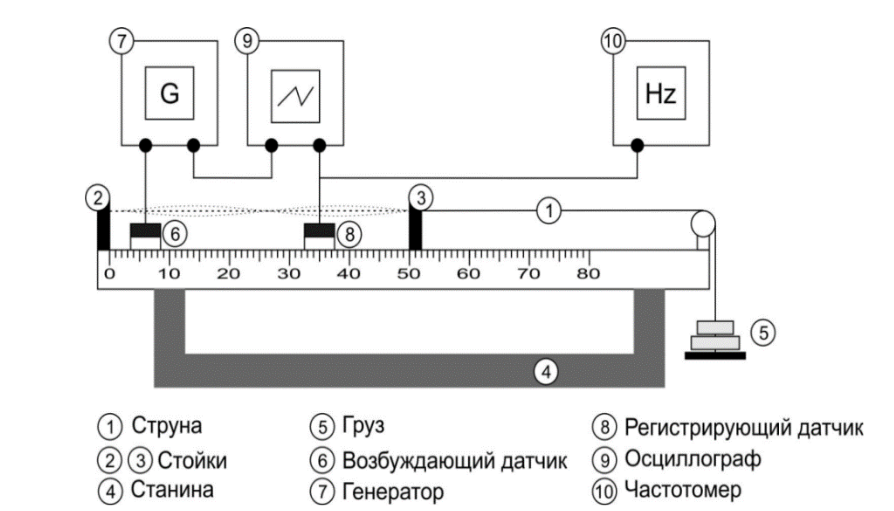
\includegraphics[scale=0.6]{схема}
\end{center}

\newpage
\section{Визуальное наблюдение стоячих волн}
\begin{itemize}
\item Установим $L = 50\text{ см}$ и положим на платформу грузы массой 487.4 г и 453.4 г, тогда суммарная масса подвеса(с учетом массы платформы и крючка, равной 119.9 г) M = 1060.7 г. На установке указано $\rho_l = 568.4 \frac{\text{мг}}{\text{м}}$, тогда:\\
\[u = \sqrt{\frac{T}{\rho_l}} = \sqrt{\frac{M\cdot g}{\rho_l}} = 133.21 \frac{\text{м}}{\text{с}}\]
\[\nu_1 = \frac{1}{2L}\cdot\sqrt{\frac{T}{\rho_l}}=133.21\text{ Гц}\]
\item Теперь включим генератор и посчитаем значение основной гармоники и более высоких гармоник при помощи осциллографа:
\[\text{Таблица №1}\]
\begin{center}
\begin{tabular}{|c|c|c|}
\hline
$\nu_{n_{exp}}\text{, Гц}$              & $\nu_{n_{theor}}\text{, Гц}$     & n \\ \hline
131.58          & 135.3  & 1     \\ \hline
246.30           & 270.0    & 2     \\ \hline
392.16 & 405.0    & 3     \\ \hline
533.12          & 541.2  & 4     \\ \hline
672.31          & 675.0    & 5     \\ \hline
798.00             & 810.0    & 6     \\ \hline
947.96          & 947.1  & 7     \\ \hline
1225.00            & 1215.0   & 9     \\ \hline
1518.00            & 1485.0   & 11    \\ \hline
1804.00            & 1758.9 & 13    \\ \hline
\end{tabular}
\end{center}
Как видим, теоретические и экспериментальные результаты с некоторой точностью совпадают.
\end{itemize}


\section{Регистрация стоячих волн с помощью осциллографа}
Проведем измерения частот гармоник для дргуих значений $M\epsilon\{1536.6\text{ г, }$ $1870.9\text{ г, }2352.7\text{ г, }2835.1\text{ г}\}$ :

\begin{center}
Таблица №1\\
\begin{tabular}{|c|c|c|c|c|c|c|c|c|c|c|}
\hline
M, г                             & n  & 1   & 2   & 3   & 4   & 5    & 6    & 7    & 8    & 9    \\ \hline
\multirow{2}{*}{1536.6}           & $\nu_{n_{exp}}\text{, Гц}$ & 160 & 328 & 485 & 654 & 815  & 983  & 1146 & 1318 & 1480 \\ \cline{2-11} 
                              & $\nu_{n_{theor}}\text{, Гц}$ & 163 & 326 & 489 & 652 & 815  & 978  & 1141 & 1304 & 1467 \\ \hline
\multirow{2}{*}{1870.9} & $\nu_{n_{exp}}\text{, Гц}$ & 182 & 366 & 548 & 735 & 915  & 1103 & 1287 & 1447 & 1659 \\ \cline{2-11} 
                              & $\nu_{n_{theor}}\text{, Гц}$ & 180 & 360 & 540 & 720 & 900  & 1080 & 1260 & 1440 & 1620 \\ \hline
\multirow{2}{*}{2352.7}          & $\nu_{n_{exp}}\text{, Гц}$ & 200 & 407 & 608 & 812 & 1013 & 1224 & 1428 & 1630 & 1839 \\ \cline{2-11} 
                              & $\nu_{n_{theor}}\text{, Гц}$ & 201 & 402 & 603 & 804 & 1005 & 1206 & 1407 & 1608 & 1809 \\ \hline
\multirow{2}{*}{2835.1}          & $\nu_{n_{exp}}\text{, Гц}$ & 223 & 449 & 668 & 898 & 1121 & 1349 & 1580 & 1802 & 2025 \\ \cline{2-11} 
                              & $\nu_{n_{theor}}\text{, Гц}$ & 221 & 442 & 663 & 884 & 1105 & 1326 & 1547 & 1768 & 1989 \\ \hline
\end{tabular}
\end{center}
\section{Наблюдение фигуры Лиссажу}
Подадим на каналы осциллографа сигналы с частотой основной гармоники $\nu_1$ и в два раза меньше $\frac{\nu_1}{2}$, тогда на экране будет наблюдаться фигура Лиссажу с одним самопересечением:
\begin{center}
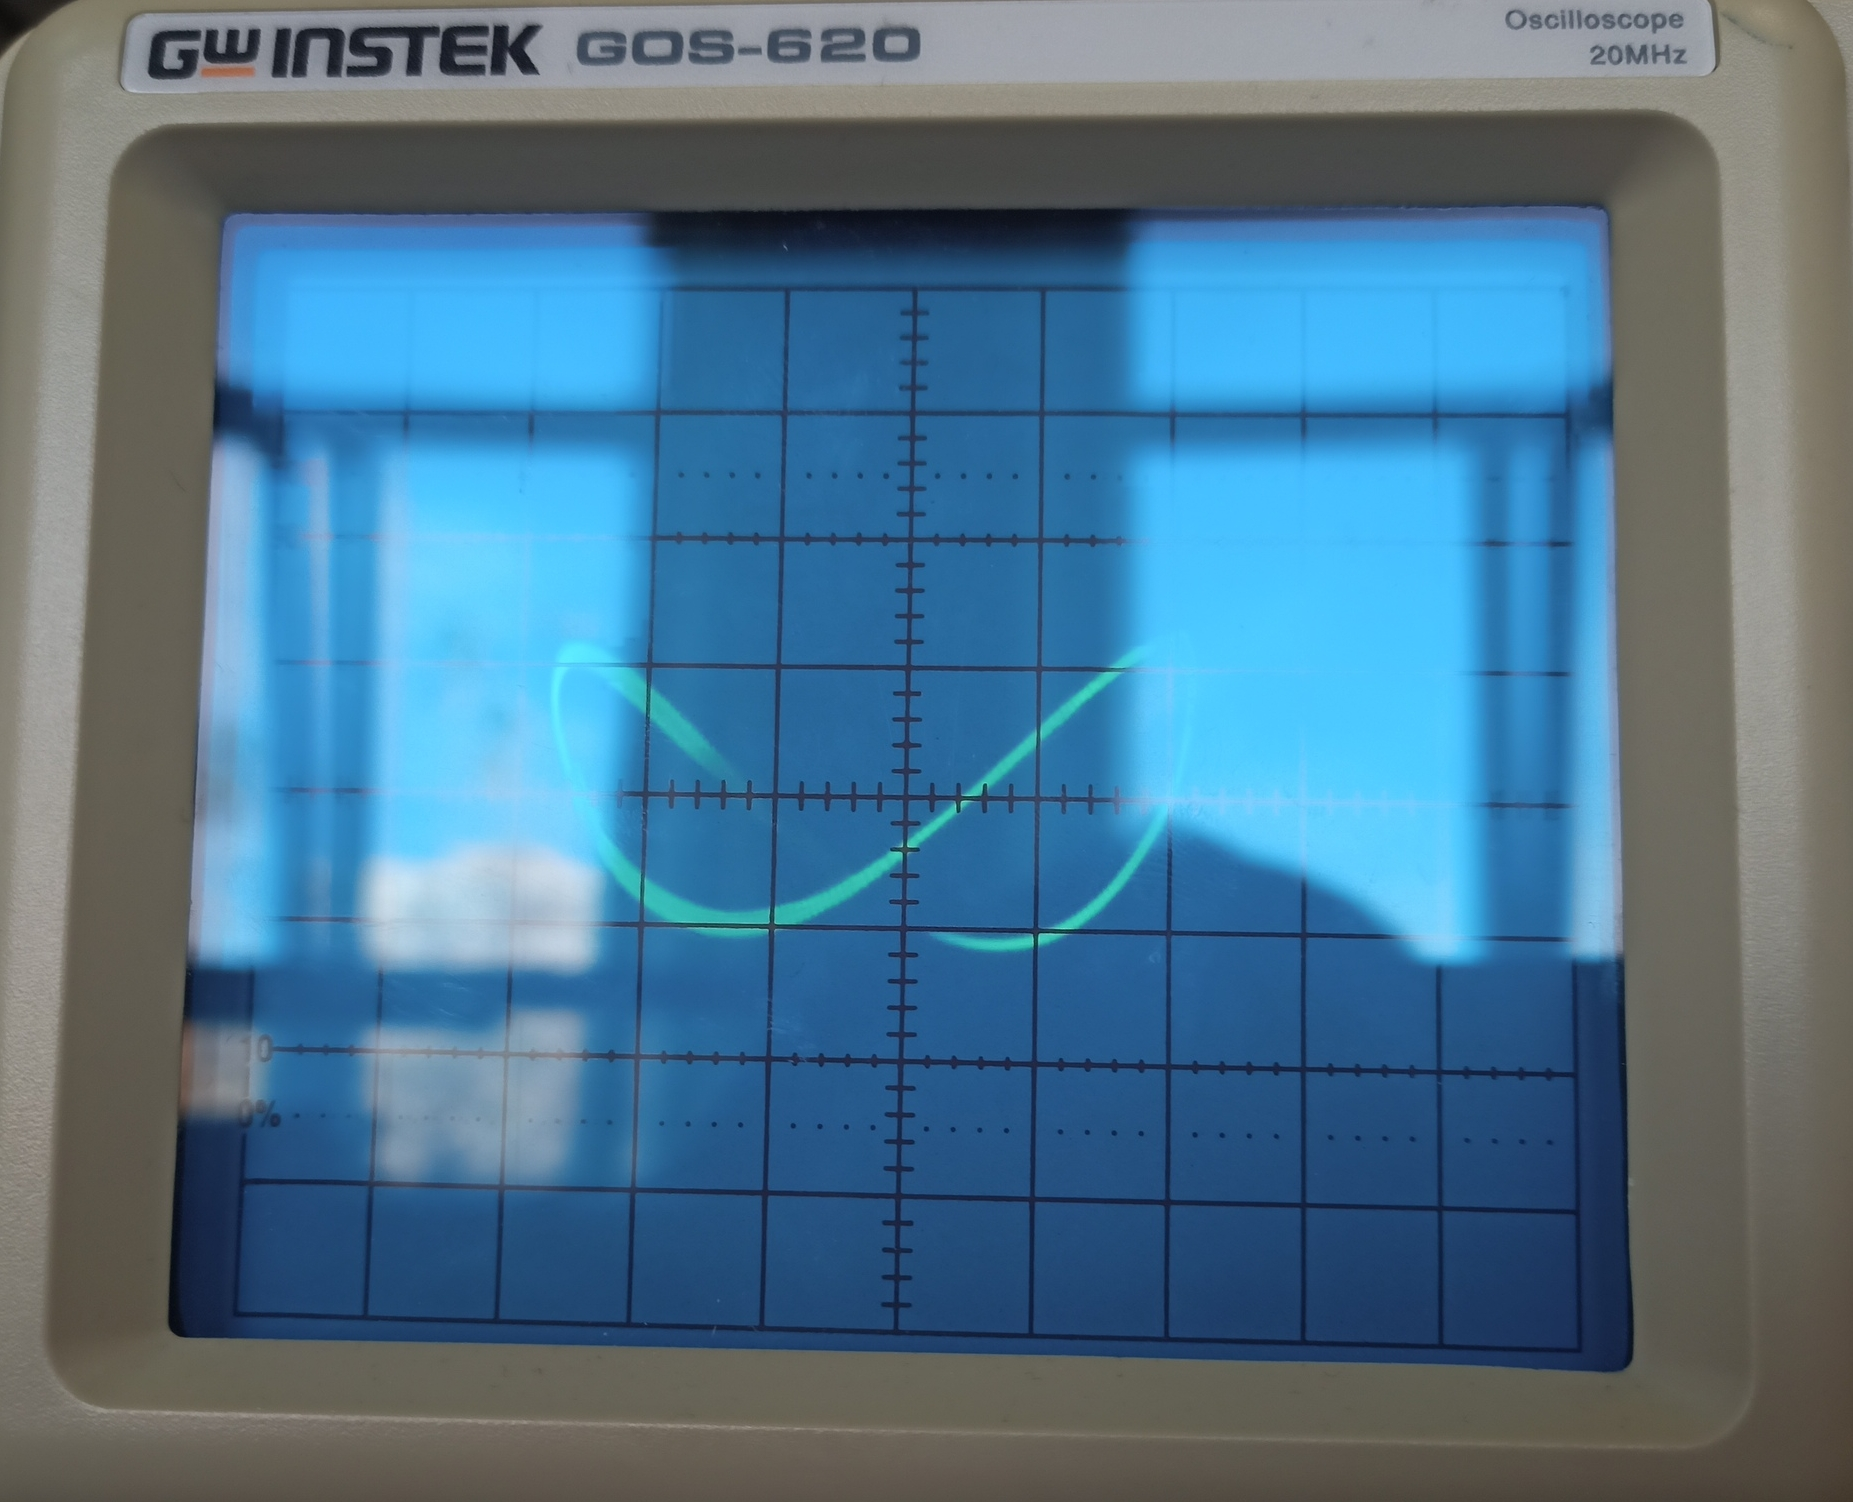
\includegraphics[scale=0.2]{lis}
\end{center}
Происходит это из-за отношения частот подаваемых сигналов, равного 1:2
\section{Определение добротности струны}
Измерим АЧХ струны вблизи частоты $\nu_1$ для M = 1060.7 г:
\begin{center}
Таблица №2\\
\begin{tabular}[h]{|c|c|}
\hline
$\nu\text{, Гц}$     & А, мВ    \\ \hline
135.0   & 5.5  \\ \hline
136.0   & 12.0   \\ \hline
136.1 & 18.0   \\ \hline
136.2 & 22.0   \\ \hline
136.3 & 40.0   \\ \hline
136.4 & 95.0   \\ \hline
136.5 & 105.0  \\ \hline
136.6 & -    \\ \hline
136.7 & 80.0   \\ \hline
136.8 & 36.0   \\ \hline
136.9 & 24.0   \\ \hline
137.0   & 18.0   \\ \hline
138.0   & 12.5 \\ \hline
\end{tabular}
\end{center}
\begin{center}
График №1\\
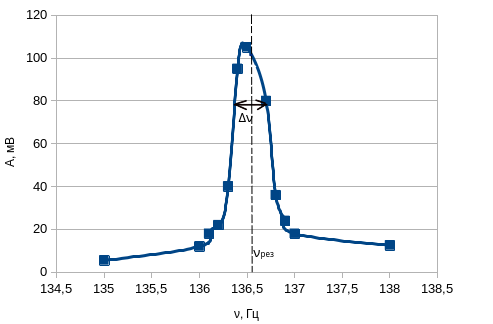
\includegraphics[scale=0.8]{graph}
\end{center}
\[\Delta\nu = 0.341 \text{ Гц; }\nu_{\text{рез}} = 136.545\text{ Гц}\]
\[Q = \frac{\nu_{\text{рез}}}{\Delta\nu} = 400.43\]

\section{Построение графиков зависимостей $\nu$ от n для разных значений силы натяжения Т и определение скорости распространения волн u  }
\begin{center}
График №2\\
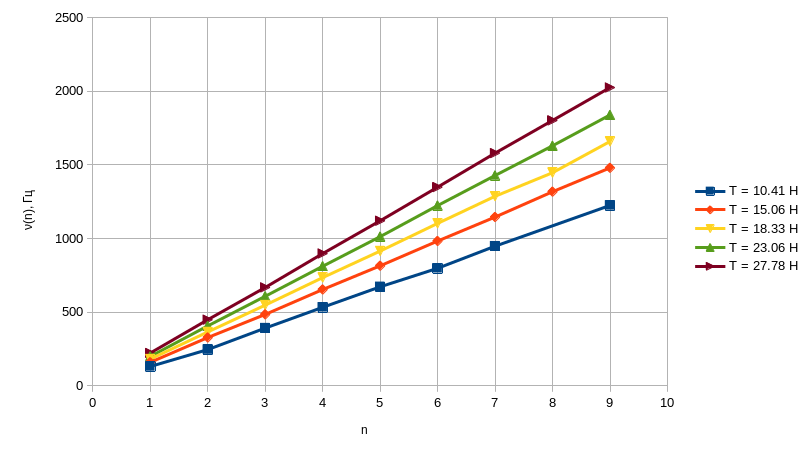
\includegraphics[scale=0.5]{graph1}
\end{center}
\[\nu = \frac{n}{2L}\cdot u\Rightarrow u(T) = k(T)\cdot 2L(\text{где k(Т) -  коэффициент наклона на графике №2})\]
\begin{center}
\begin{tabular}{|c|c|c|c|c|}
\hline
$\text{T, H}$     & $\text{k, Гц}$      & $\varepsilon_k$    & $\text u, \frac{\text{м}}{\text{с}}$     & $\Delta u \text{, }\frac{\text{м}}{\text{с}}$   \\ \hline
10.41 & 137.66 & 0.011 & 137.7 & 1.5 \\ \hline
15.06 & 165.02 & 0.012 & 165.0 & 2.0 \\ \hline
18.33 & 183.28 & 0.014 & 183.3 & 2.6 \\ \hline
23.06 & 204.62 & 0.015 & 204.6 & 3.1 \\ \hline
27.78 & 225.70 & 0.017 & 225.7 & 3.8 \\ \hline
\end{tabular}
\end{center}


\section{Определение $\rho_l$}
\[u = \sqrt{\frac{T}{\rho_l}} \Rightarrow T = \rho_l \cdot u^2\]
\[\Delta (u^2) = u^2 \cdot\sqrt{2\cdot \left( \frac{\Delta u}{u}\right)^2}\]
\begin{center}
\begin{tabular}{|c|c|c|c|}
\hline
T, H     & $u^2$, $\left(\frac{\text{м}}{\text{c}}\right)^2$     & $u$, $\frac{\text{м}}{\text{с}}$     & $\Delta (u^2)$, $\left(\frac{\text{м}}{\text{c}}\right)^2$   \\ \hline
10.41 & 18961 & 137.7 & 295  \\ \hline
15.06 & 27225 & 165.0 & 462  \\ \hline
18.33 & 33599 & 183.3 & 705  \\ \hline
23.06 & 41861 & 204.6 & 888  \\ \hline
27.78 & 50940 & 225.7 & 1225 \\ \hline
\end{tabular}
\end{center}
\begin{center}
График №3
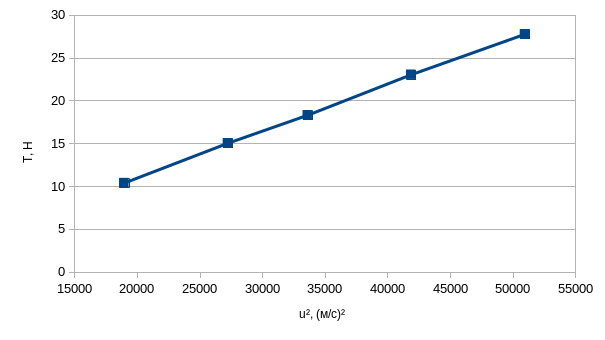
\includegraphics[scale=0.6]{graph2}
\end{center}
Из графика получаем $\rho_l = k = (563.8\pm22.4)\frac{\text{мг}}{\text{м}}$

Как видим,результат эксперимента согласуется с данными, указанными на установке.
\end{document}